\section{Problem 4}

\subsection{Question}
Compute the Kendall Tau\_b score for both lists (use \enquote{b} because
there will likely be tie values in the rankings).  Report both the
Tau value and the \enquote{p} value.\\
\\
See:\\ 
http://stackoverflow.com/questions/2557863/measures-of-association-in-r-kendalls-tau-b-and-tau-c\\
http://en.wikipedia.org/wiki/Kendall\_tau\_rank\_correlation\_coefficient\#Tau-b\\
http://en.wikipedia.org/wiki/Correlation\_and\_dependence\\



\subsection{Answer}
\vspace{2mm}
Using R, I input the values of TFIDF and Page rank into two separate vectors.
Using the package\cite{package} Kendall\cite{kendall}, it calculated a tau of 0.866 and p of 0.0018457.
With a tau number so close to +1, there is a high association between the two measured quantities.
In the case of ties, both packages \enquote{Kendall and cor produce the same result but cor.test produces a p-value which is not as accurate}.
\vspace{5mm}
\lstinputlisting[language=R, caption={kendall.r}, label=listing:kendall.r]{q4/kendall.r}
\vspace{5mm}
\begin{figure}[h]
\centering
\fbox{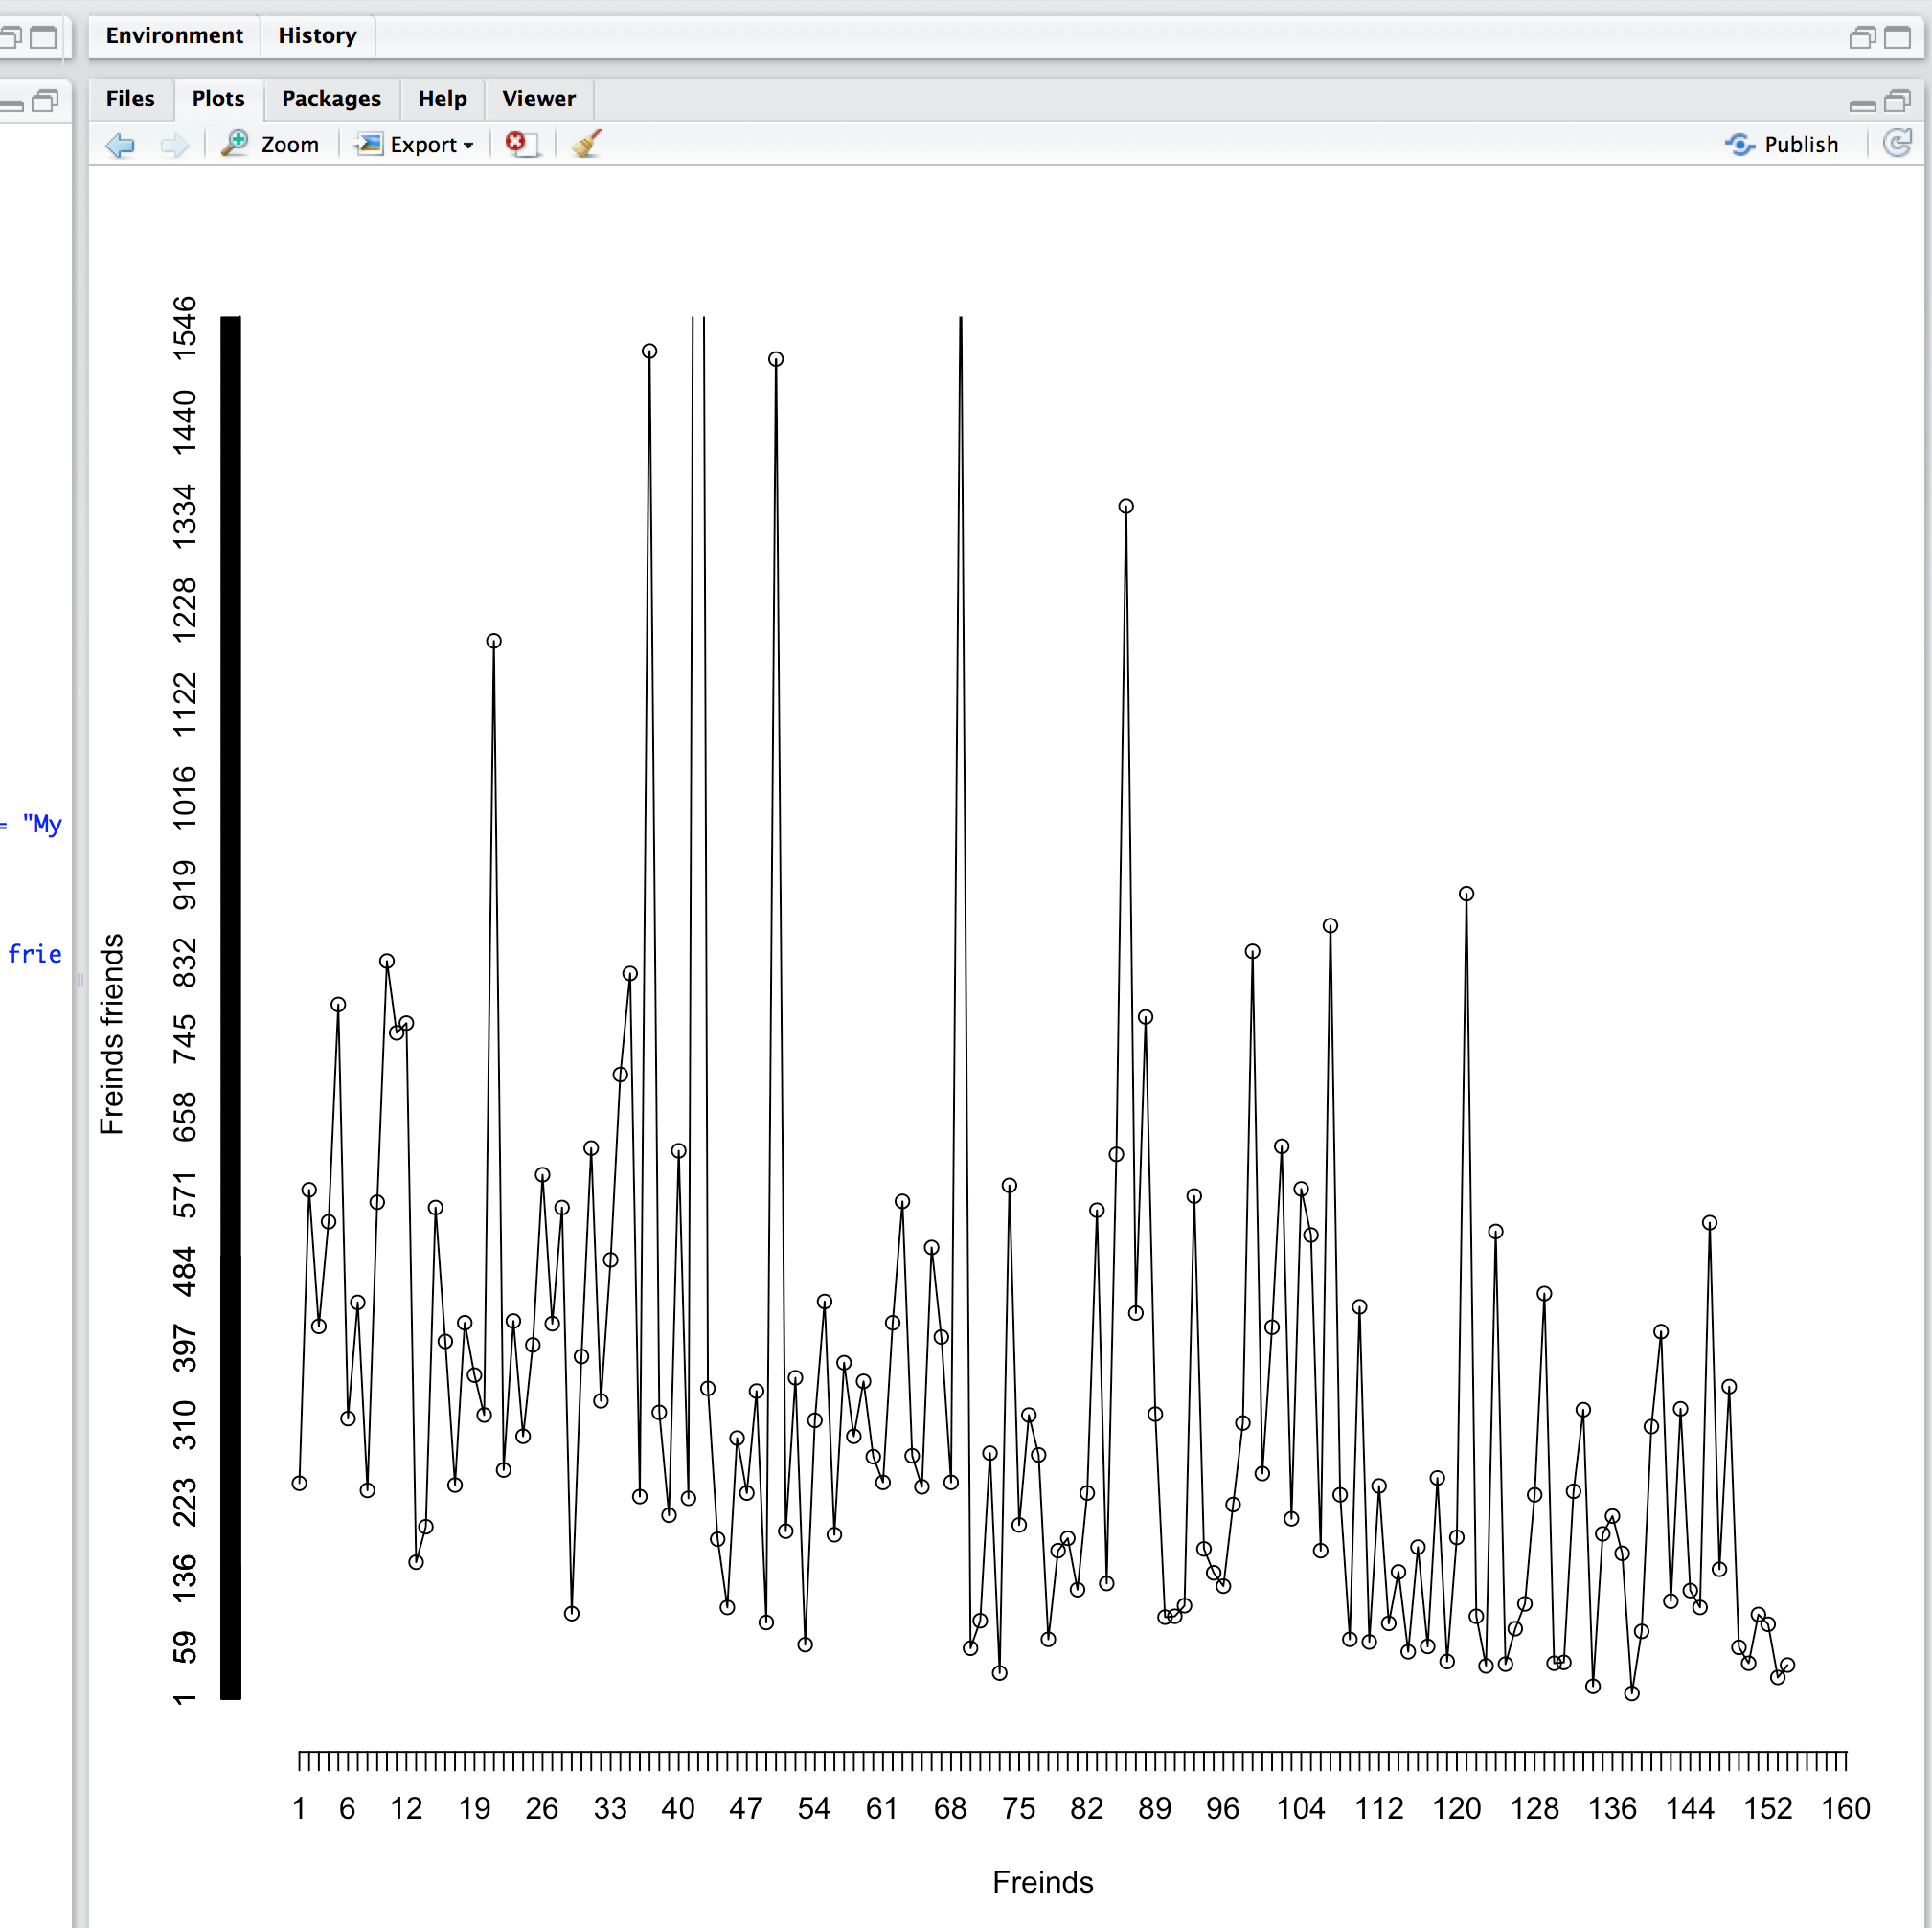
\includegraphics[scale=.95]{q4/fig1.png}}
\caption{R script that computes the Tau and p value of the Kendall Tau correlation}
\label{fig:fig1}
\end{figure}
\newpage
\vspace{5mm}
\begin{figure}[h]
\centering
\fbox{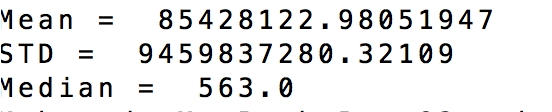
\includegraphics[scale=.95]{q4/fig2.png}}
\caption{Tau and p value of the Kendall}
\label{fig:fig2}
\end{figure}

